\makeatletter
  \graphicspath{ {\import@path} }
\makeatother

%%%%%%%%%%%%%%%%%%%%%%%%%%%%%%%%%%%%%%%%%%%%%%%%%%%%%%%%%%%%%%%%%%%%%%%%%%%%%%%
\begin{frame}[fragile]{Benchmark: Kinematic Likelihood Fitting}
  \begin{itemize}
    \item[$\bullet$]
        Kinematic likelihood fitting is performed as a baseline study,
        the \href{https://github.com/KLFitter/KLFitter}{\textsc{KLFitter}} library is used.
        {\scriptsize \href{https://www.sciencedirect.com/science/article/pii/S0168900214001855?via\%3Dihub}{[J. Erdmann, Nucl.Instrum.Meth.A 748 (2014) 18-25]}}
        \scalebox{.7}{$
            \mathcal{L} = B(m_{q_{1}q_{2}q_{3}}|m_{t},\Gamma_{t}) \cdot
                         B(m_{q_{1}q_{2}}|m_{W},\Gamma_{W}) \cdot
                         B(m_{q_{4}q_{5}q_{6}}|m_{t},\Gamma_{t}) \cdot
                         B(m_{q_{4}q_{5}}|m_{W},\Gamma_{W}) \cdot
                         \prod_{i=1}^{6} W_{\text{jet}}(E_{\text{jet},i}^{\text{meas}}|E_{\text{jet},i})
        $},
        {\footnotesize where $B$ indicates the Breit-Wigner distribution and $W$ does the the transfer functions}
    \smallskip

    \item[$\bullet$]
        As more jets are used, the number of permutations increases explosively.
        Therefore, two case are studied.
              \begin{itemize}
                  \item[-] Most energetic 6 jets, $N_{jets}^{in} = 6 \rightarrow $ Avg. 18 permutations
                  \item[-] Up to 7 most energetic jets $N_{jets}^{in} \leq 7 \rightarrow$  Avg. 126 permutations
              \end{itemize}
    \smallskip

    \item[$\bullet$]
        When the best permutation has a likelihood lower than the threshold, the event is not selected.
  \end{itemize}

\end{frame}



%%%%%%%%%%%%%%%%%%%%%%%%%%%%%%%%%%%%%%%%%%%%%%%%%%%%%%%%%%%%%%%%%%%%%%%%%%%%%%%%
\begin{frame}[fragile]{Predictive entropy distribution}
    \begin{figure}
        \centering
        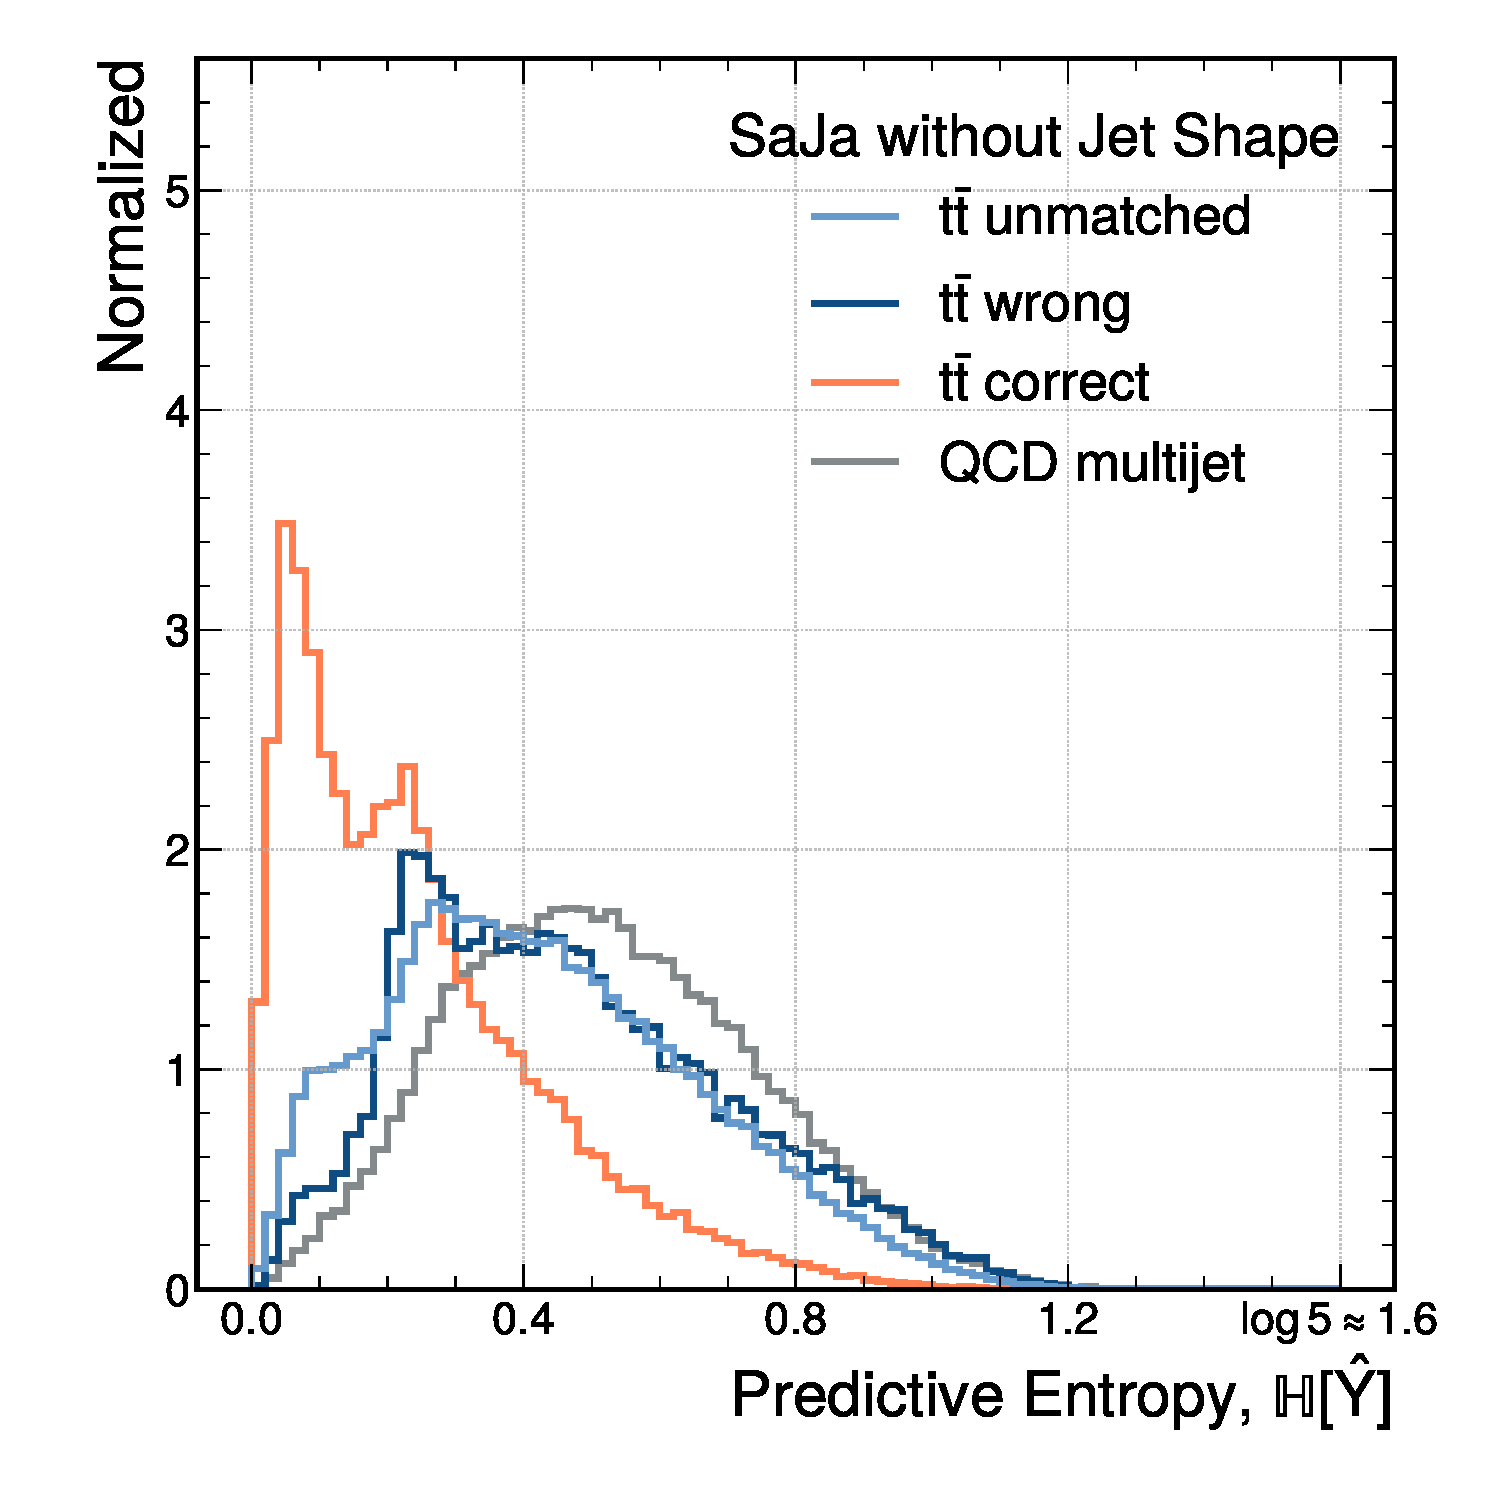
\includegraphics[width=0.45\textwidth]{fig/entropy/entropy-without-jet-shape.pdf}
        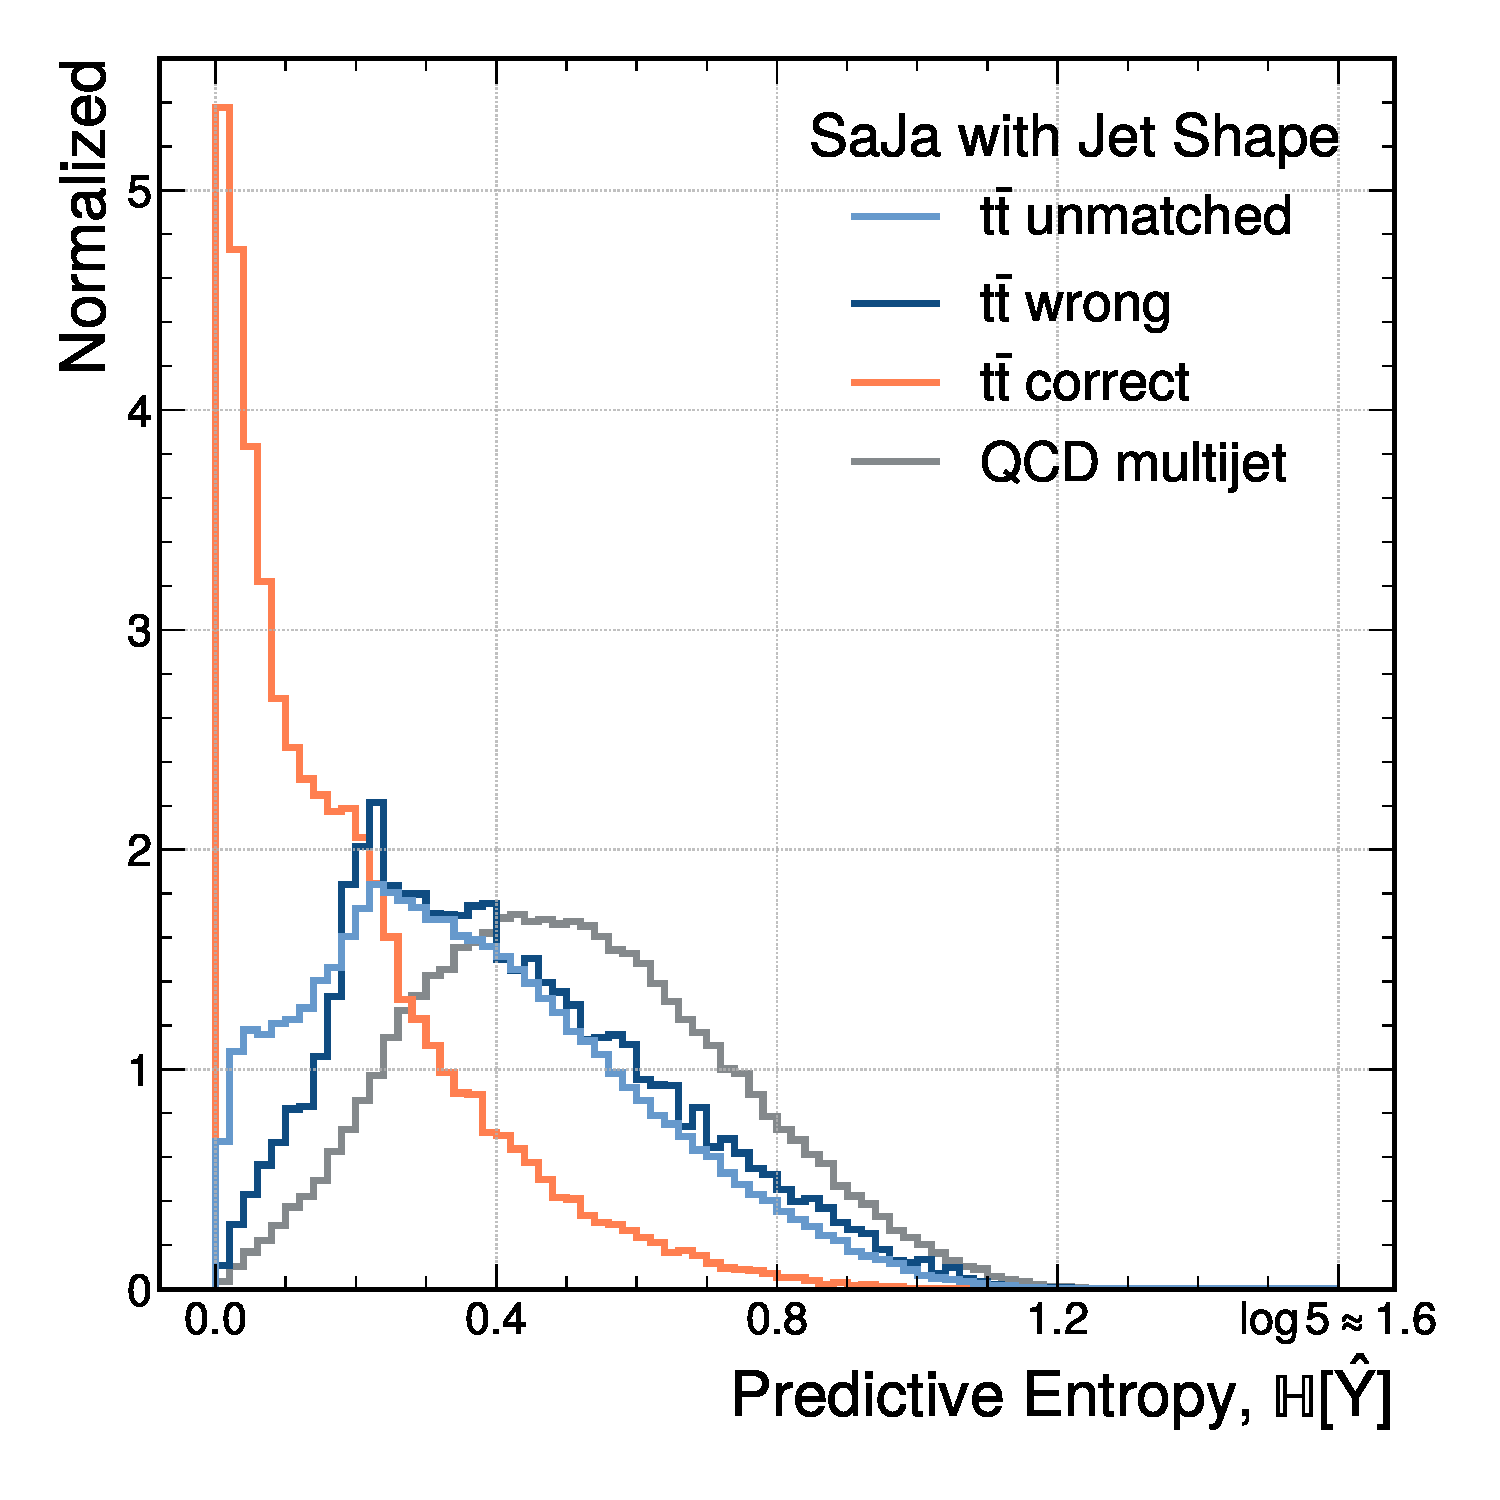
\includegraphics[width=0.45\textwidth]{fig/entropy/entropy-with-jet-shape.pdf}
    \end{figure}
\end{frame}

\begin{frame}[fragile]{Effect of Jet Shape}
    \begin{figure}
        \centering
        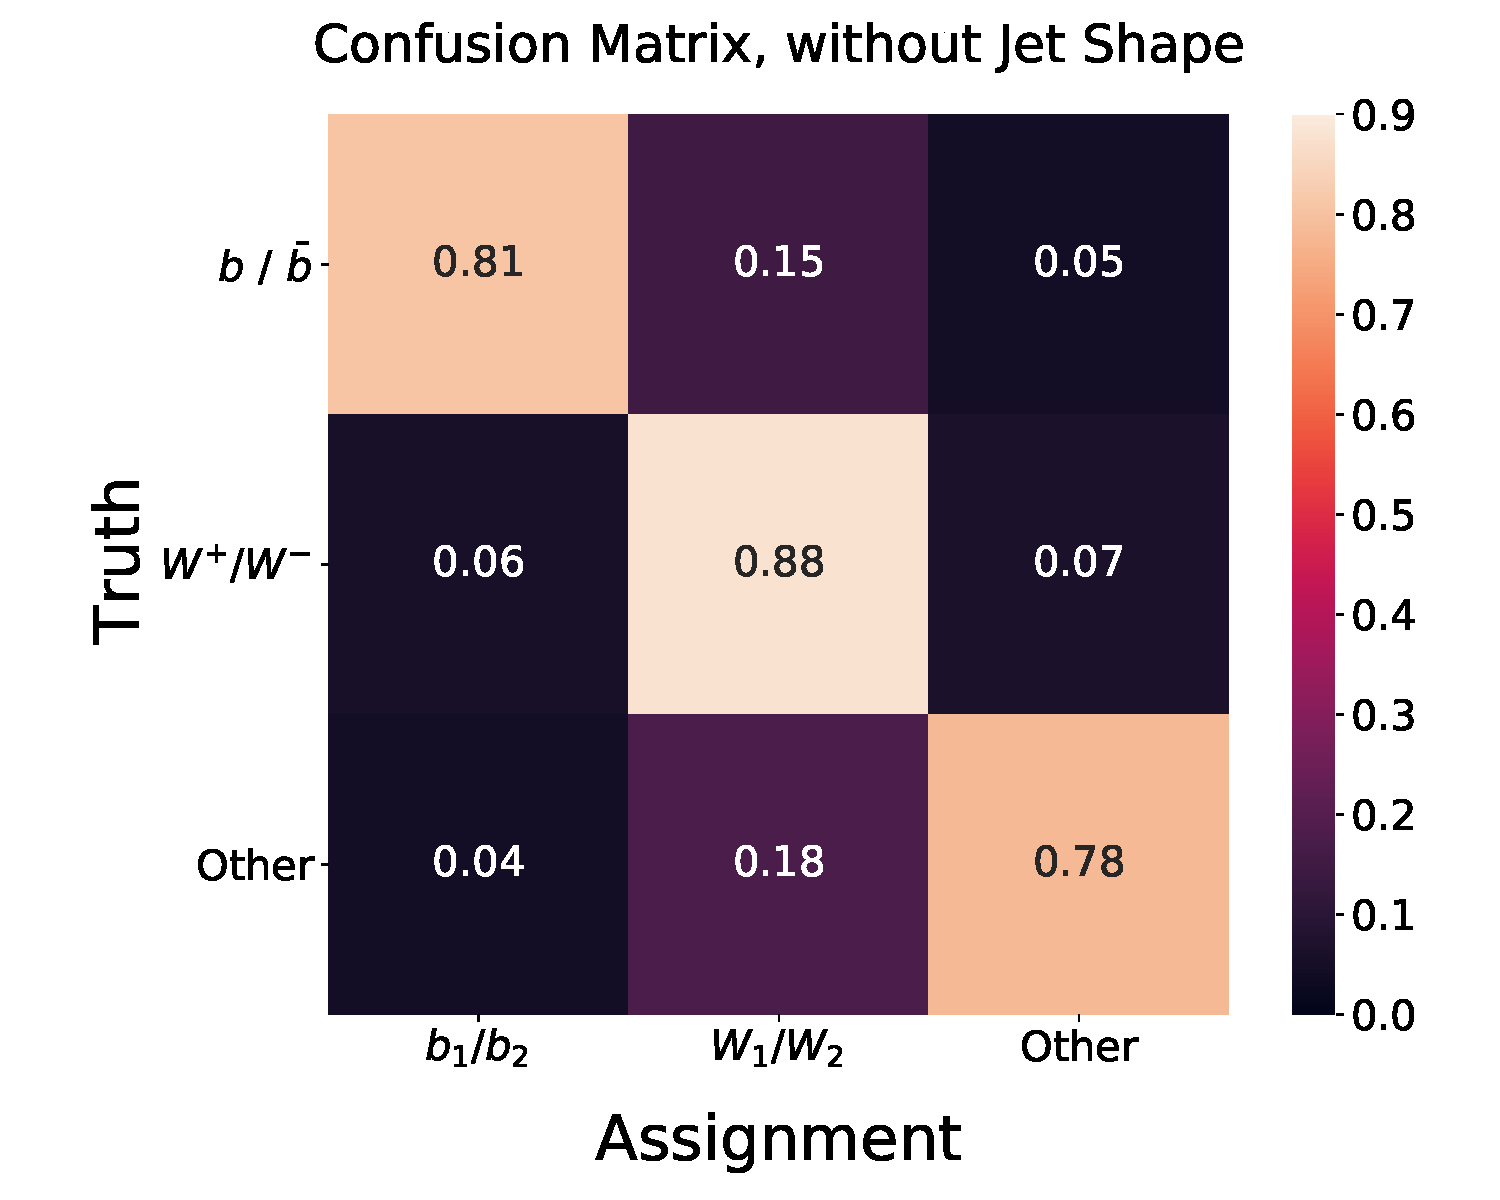
\includegraphics[width=0.45\textwidth]{fig/confusion-matrix/confusion_matrix_without_jet_shape.pdf}
        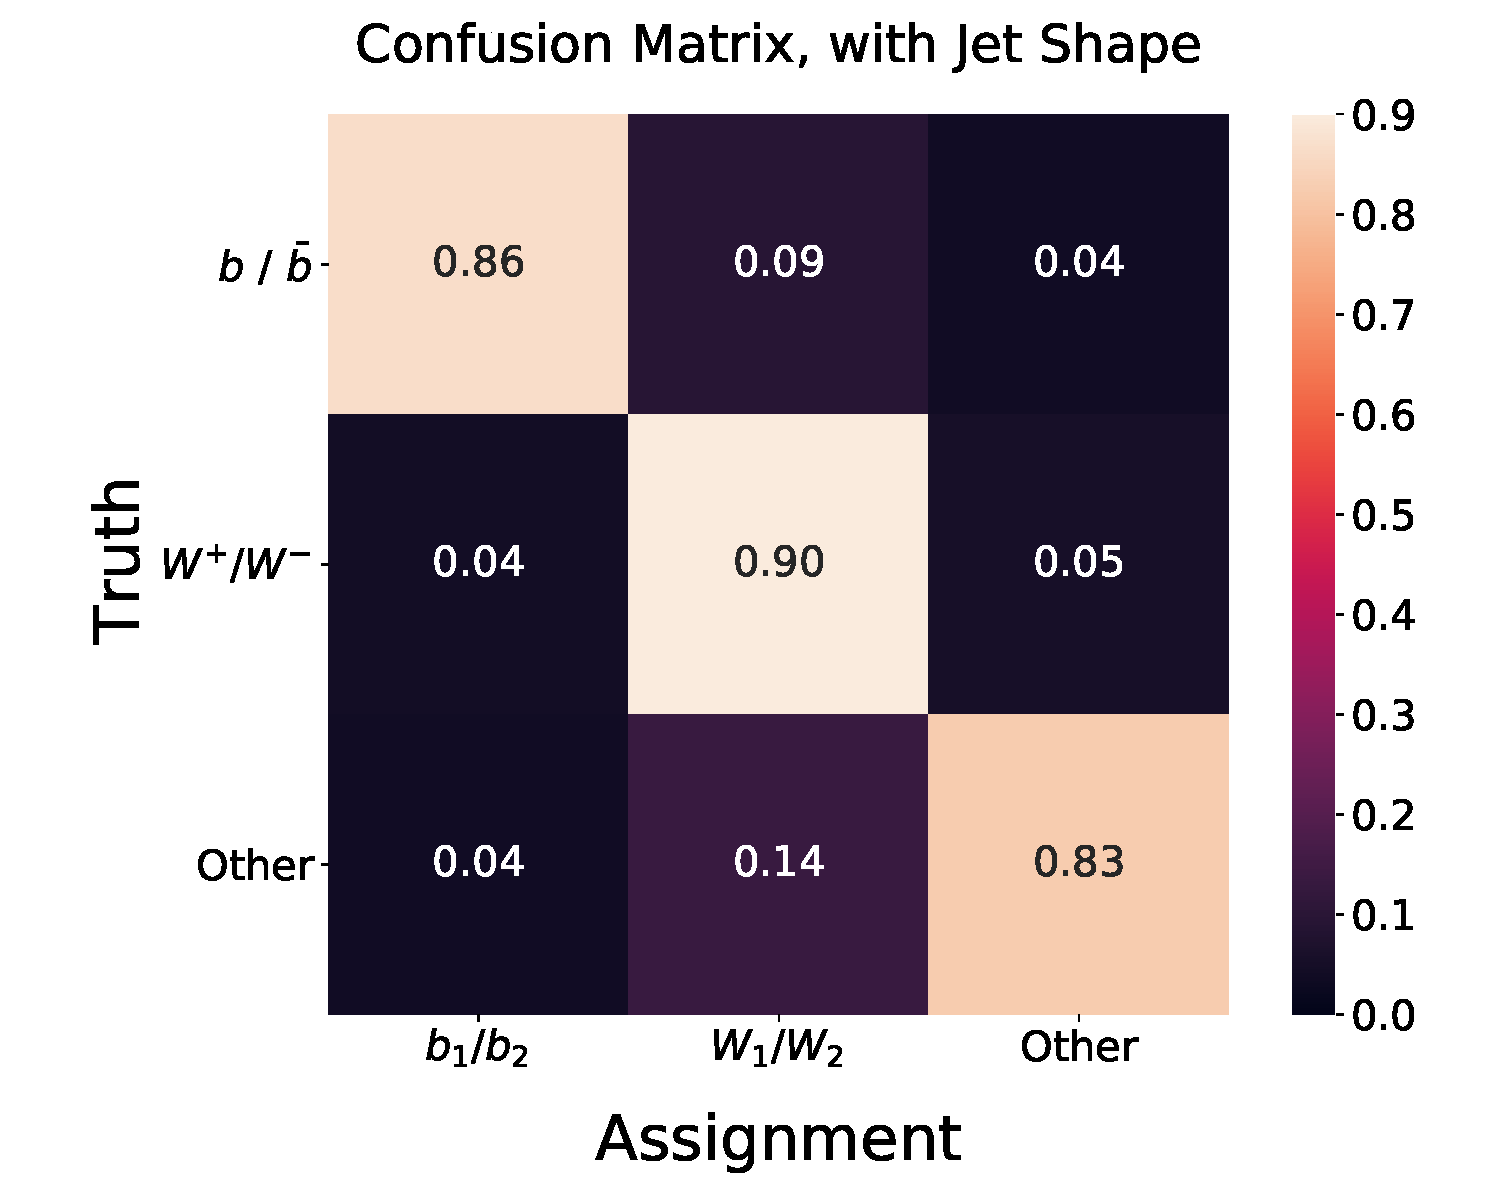
\includegraphics[width=0.45\textwidth]{fig/confusion-matrix/confusion_matrix_with_jet_shape.pdf}
    \end{figure}
    Jet shape reduces the case where b-initiated jets and additional jets are assigned to W boson.
\end{frame}

\begin{frame}[fragile]{Fraction of Topologically Valid Assignments}
  \begin{figure}
    \centering
    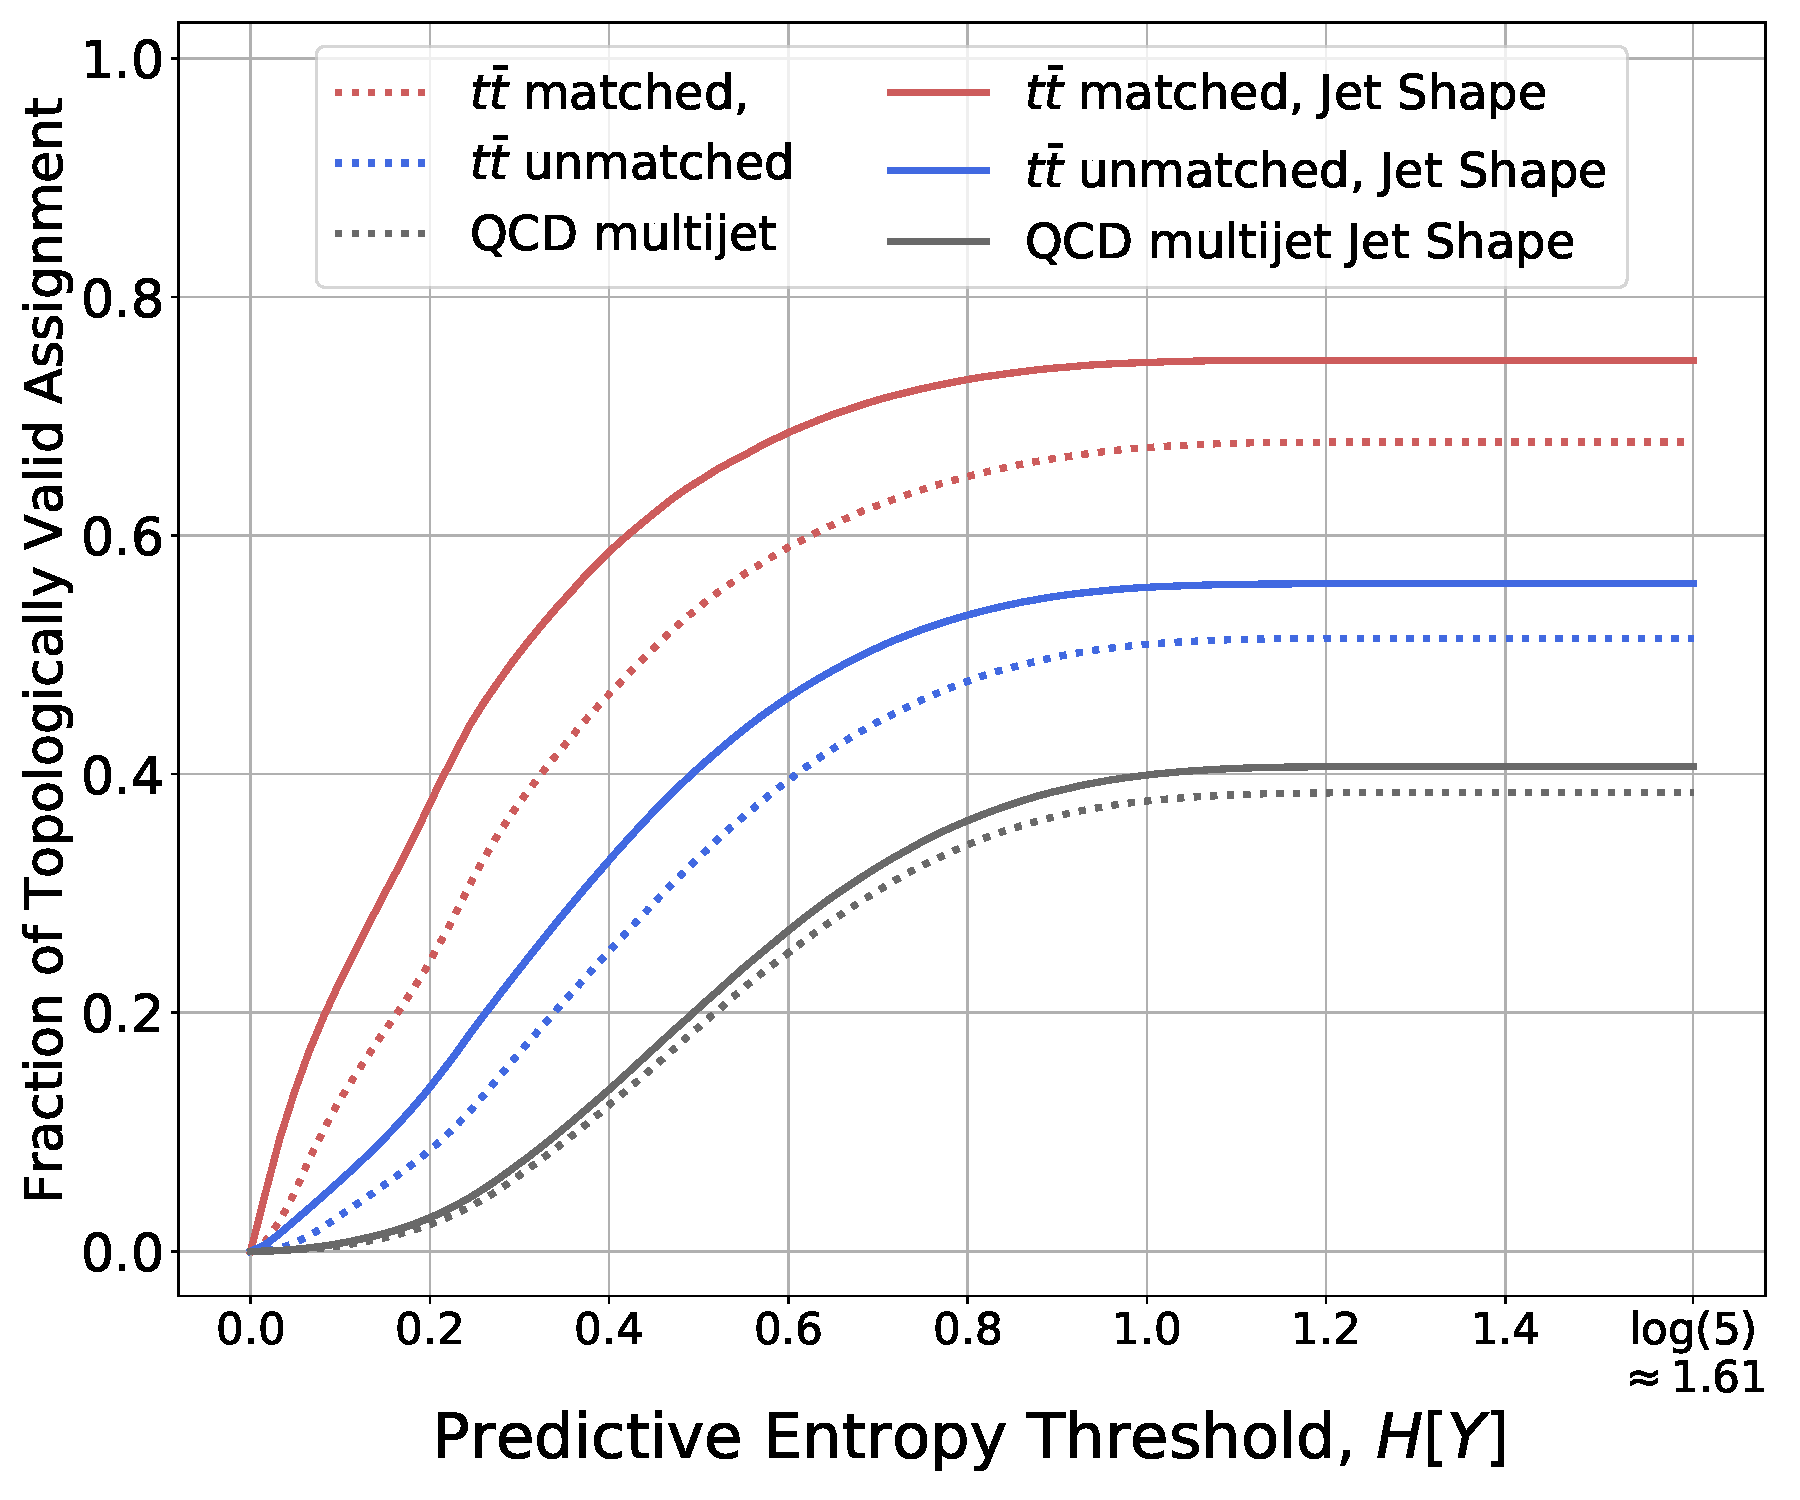
\includegraphics[width=0.8\textwidth]{fig/topo-valid/frac_topo_valid.pdf}
  \end{figure}
\end{frame}

\begin{frame}[fragile]{Training in detail}
  \begin{itemize}
    \item Training, validation, test set: 311k, 80k, 103k events
    \item Adam Optimization algorithm
    \item Learning rate schedule, which reduces the learning rate when the metric on the validation set has stopped improving.
      \item \textsc{PyTorch} v1.3
  \end{itemize}
\end{frame}

\begin{frame}[fragile]{Reconstructed W Boson and Top Quark Mass Distributions}
    \begin{figure}
        \centering
        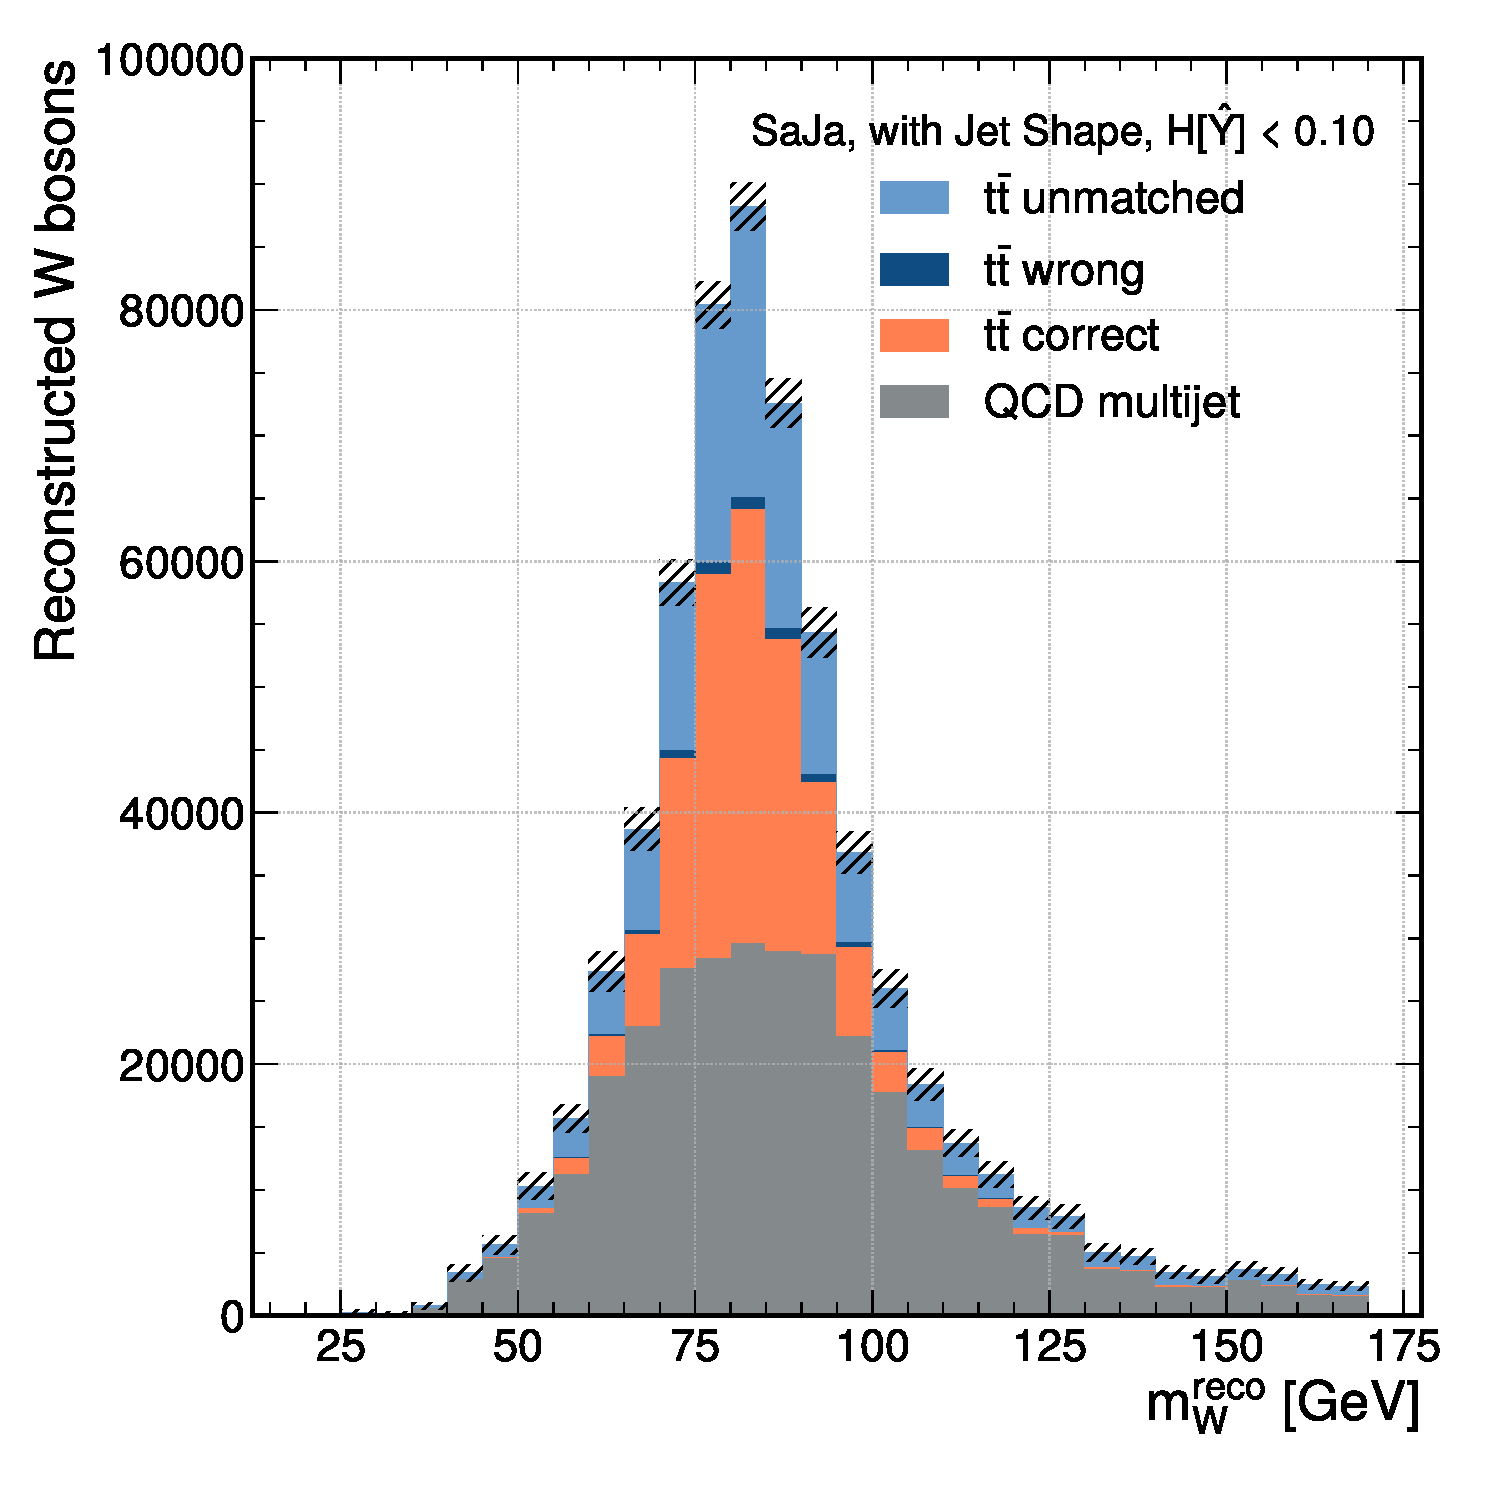
\includegraphics[width=0.48\textwidth]{fig/reco/w-mass_entropy-cut-0.10.pdf}
        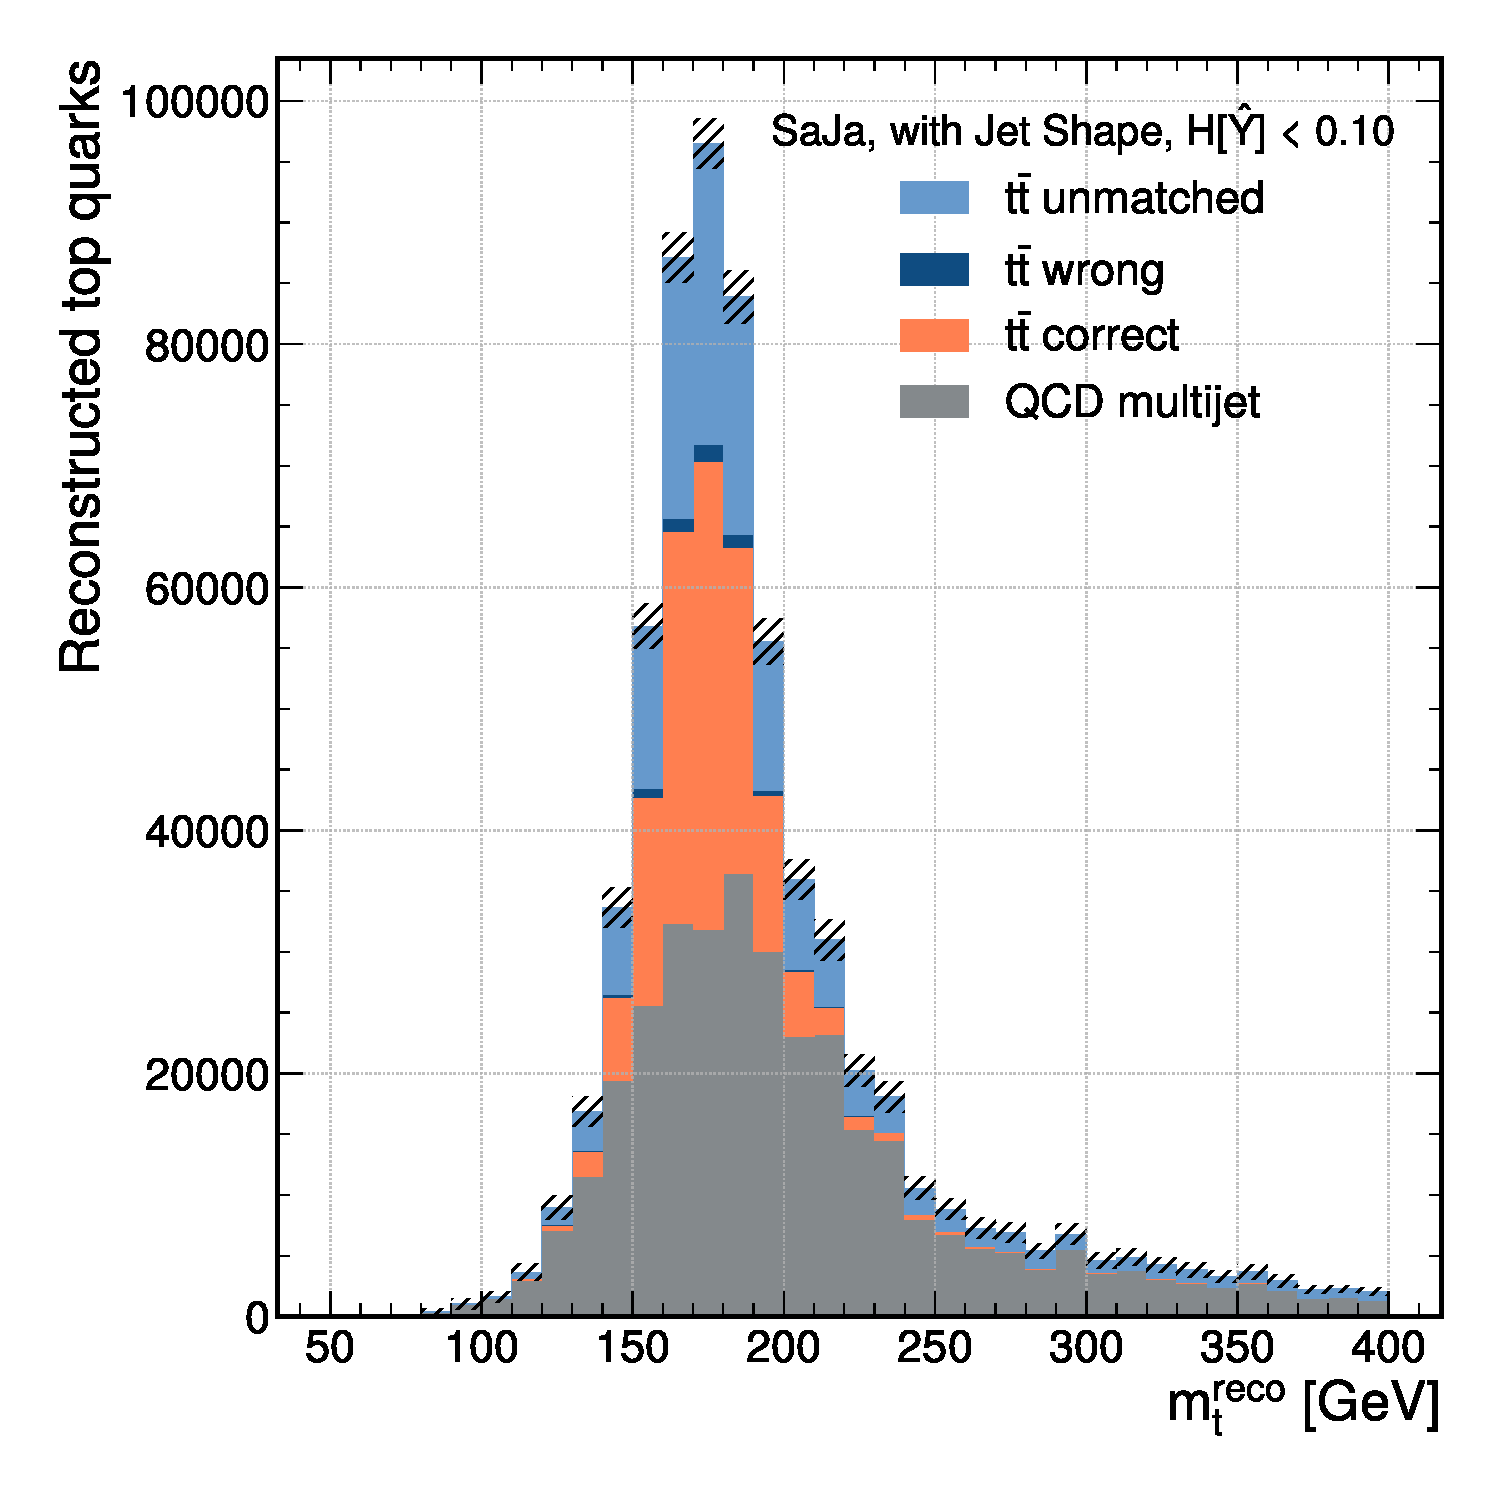
\includegraphics[width=0.48\textwidth]{fig/reco/top-mass_entropy-cut-0.10.pdf}
    \end{figure}
    (Left) Reconstructed W boson mass distribution and (Right) reconstructed top quark mass distribution.
\end{frame}

